\documentclass{beamer}
 \usepackage{hyperref}
\usepackage[frenchb]{babel}
\usepackage[latin1]{inputenc}
\usepackage{ucs}
\usepackage{lmodern}
\usefonttheme{serif,professionalfonts}
\usepackage{amsfonts}
\usepackage{tkz-tab}
\usepackage{cancel}
\usepackage{tkz-base,tkz-fct}
\definecolor{myred}{rgb}{0.93,0.26,0}
\usepackage{pst-text,pst-plot,pst-math,pst-tree}
\usepackage{mathrsfs}
\usepackage{color}
%\usepackage{colortbl}
\usepackage{multicol}
\newcommand{\R}{\mathbb{R}}
\newcommand{\C}{\mathbb{C}}
\newcommand{\N}{\mathbb{N}}
\newcommand{\Z}{\mathbb{Z}}
\newcommand{\Q}{\mathbb{Q}}
\newcommand{\D}{\mathbb{D}}\newcommand{\vect}[1]{\overrightarrow{\,\mathstrut#1\,}}
\newsavebox{\fmbox}

\newenvironment{encadrer}{%
	\vspace{1em}
    \begin{lrbox}{\fmbox}\begin{minipage}{0.98\textwidth}}
    {%\vspace{1em}
    \end{minipage}\end{lrbox}\fbox{\usebox{\fmbox}}
	
	\vspace{1em}
	}
\everymath{\displaystyle}
\usepackage{tabularx}
\usepackage{pifont}
\usepackage{ifthen}
\usepackage{amsmath,multicol}
\usepackage{fancybox,color}
\usepackage{xcolor}
\usepackage[pstricks]{bclogo}
\usepackage{pstricks,pst-node,pst-text,pst-coil}
\setcounter{tocdepth}{1} %\setcounter{page}{0}
%\setcounter{page}{0}
\setbeamertemplate{section in toc}[sections numbered]

%\renewcommand\FancyVerbFormatLine[1]{\colorbox{green}{#1}}

%\usecolortheme[rgb=0.97,0.35,0.04]{structure}
\usepackage{caption}
\usecolortheme{dolphin}
\useoutertheme{shadow}
\captionsetup{labelformat=empty,font=footnotesize}


\usetheme{CambridgeUS}
  % or ...Warsaw




\begin{document}



%\subtitle{Seconde 5}



\begin{frame}
\frametitle{Exercice 2}
\setbeamertemplate{item}[circle]
\setbeamercolor{item}{fg=red}

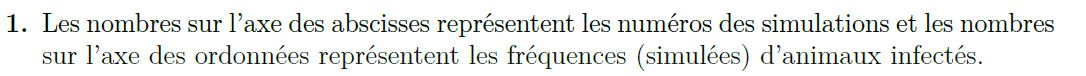
\includegraphics[scale=0.45]{conf1.jpg}
\end{frame}


\begin{frame}
\frametitle{Exercice 2}
\setbeamertemplate{item}[circle]
\setbeamercolor{item}{fg=red}


\includegraphics[scale=0.45]{conf2.jpg}
\end{frame}


\begin{frame}
\frametitle{Exercice 2}
\setbeamertemplate{item}[circle]
\setbeamercolor{item}{fg=red}


\includegraphics[scale=0.45]{conf3.jpg}
\end{frame}




\begin{frame}
\frametitle{Exercice 2}
\setbeamertemplate{item}[circle]
\setbeamercolor{item}{fg=red}

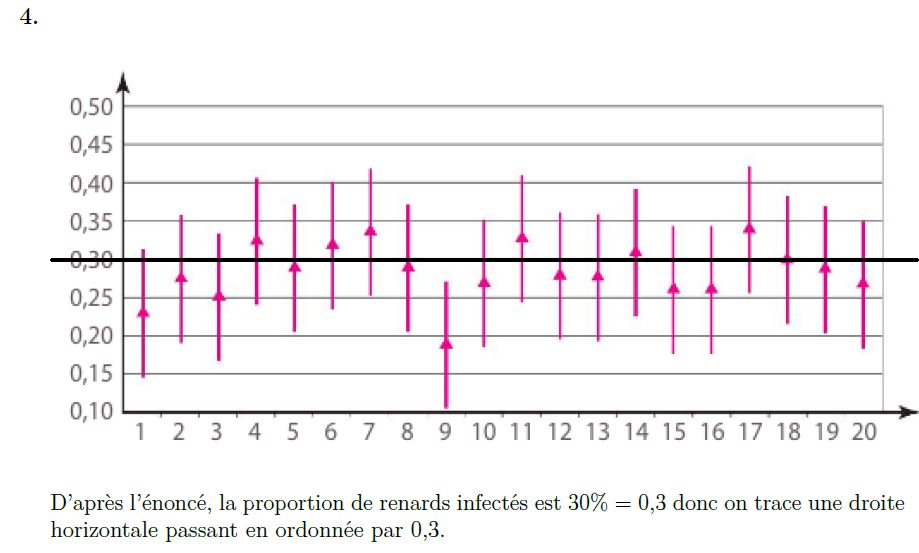
\includegraphics[scale=0.45]{conf4.jpg}
\end{frame}

\begin{frame}
\frametitle{Exercice 2}
\setbeamertemplate{item}[circle]
\setbeamercolor{item}{fg=red}

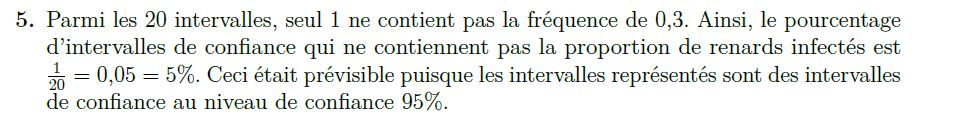
\includegraphics[scale=0.45]{conf5.jpg}
\end{frame}

\begin{frame}
\frametitle{Exercice 2}
\setbeamertemplate{item}[circle]
\setbeamercolor{item}{fg=red}

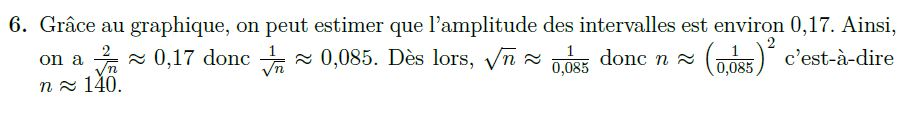
\includegraphics[scale=0.45]{conf6.jpg}
\end{frame}
\end{document}